\chapter{Case Study: Learning a Decision Tree for a Grid World with Reinforcement Learning}
\epigraphhead[30]{\selectlanguage{english}\epigraph{I have not failed. I've
    just found 10.000 ways that won't work.}{Thomas A. Edison}}

\section{The classical Grid World Markov Decision Problem}
\subsection{The Grid World MDP}
We consider a 2×2 grid world Markov Decision Process (MDP) defined as follows:
\begin{itemize}
    \item \textbf{States}: Four cells labeled $S_0$, $S_1$, $S_2$, and $G$ (goal state) arranged in a 2×2 grid.
    \item \textbf{Actions}: At each state, the agent can move right ($\rightarrow$) or down ($\downarrow$) up ($\uparrow$) or left ($\leftarrow$).
    \item \textbf{Transitions}: Movements are deterministic, following the direction of the chosen action. Actions that would lead outside the grid leave the agent in the same state.
    \item \textbf{Rewards}: All transitions yield a reward of 0, except for any action taken from the goal state $G$, which yields a reward of 1.
    \item \textbf{Objective}: Maximize the expected discounted cumulative reward.
\end{itemize}

\begin{figure}[ht]
\centering
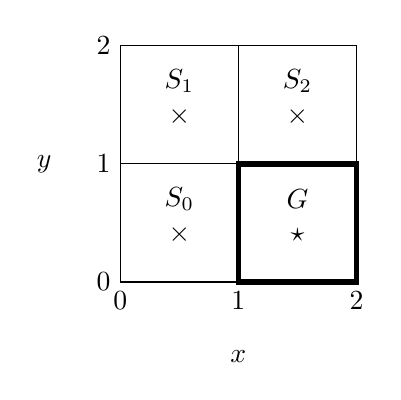
\begin{tikzpicture}[scale=1.5]
    % Draw the grid cells
    \draw (0,0) grid (2,2);
    
    % Add ticks on axes
    \foreach \x in {0,1,2}
        \node[below] at (\x,0) {$\x$};
    \foreach \y in {0,1,2}
        \node[left] at (0,\y) {$\y$};
    
    \node[left] at (-0.5, 1) {$y$};
    \node[below] at (1, -0.5) {$x$};
    
    % Label cells
    \node at (0.5,0.7) {$S_0$};
    \node at (0.5,0.4) {$\times$};

    \node at (0.5,1.7) {$S_1$};
    \node at (0.5,1.4) {$\times$};

    \node at (1.5,1.7) {$S_2$};
    \node at (1.5,1.4) {$\times$};

    
    % Goal state in bottom right with double border
    \draw[line width=2pt] (1,0) rectangle (2,1);
    \node at (1.5,0.7) {$G$};
    \node at (1.5,0.4) {$\star$};

    
\end{tikzpicture}
\caption{The 2×2 grid world environment with states $S_0$, $S_1$, $S_2$, and goal state $G$.}\label{fig:grid-world}
\end{figure}

\subsection{An optimal tabular policy}
\begin{figure}[ht]
\centering
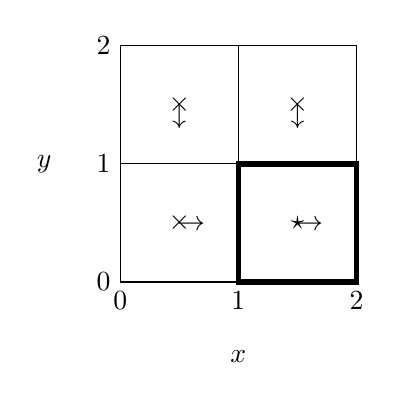
\begin{tikzpicture}[scale=1.5]
    % Draw the grid cells
    \draw (0,0) grid (2,2);
    
    % Add ticks on axes
    \foreach \x in {0,1,2}
        \node[below] at (\x,0) {$\x$};
    \foreach \y in {0,1,2}
        \node[left] at (0,\y) {$\y$};
    
    \node[left] at (-0.5, 1) {$y$};
    \node[below] at (1, -0.5) {$x$};
    
    % Label cells
    \node at (0.5,0.5) {$\times$};
    \node at (0.6,0.48) {$\rightarrow$};

    \node at (0.5,1.5) {$\times$};
    \node at (0.5,1.4) {$\downarrow$};

    \node at (1.5,1.5) {$\times$};
    \node at (1.5,1.4) {$\downarrow$};
    
    % Goal state in bottom right with double border
    \draw[line width=2pt] (1,0) rectangle (2,1);
    \node at (1.5,0.5) {$\star$};
    \node at (1.6,0.48) {$\rightarrow$};

    
\end{tikzpicture}
\caption{The optimal tabular policy for the grid world, with actions highlighted in green. This policy maps each state directly to its optimal action.}\label{fig:optimal-policy}
\end{figure}

\subsection{Some decision tree policies}

In this chapter, we explore different policy representations for the $2\times2$ grid world MDP shown in Figure~\ref{fig:grid-world}. The optimal policy for this environment can be represented in a tabular form, as shown in Figure~\ref{fig:optimal-policy} where the optimal actions at each state are highlighted in green. This tabular policy directly maps each state to its optimal action: moving right from $S_0$, down from $S_1$ and $S_2$, and right from the goal state $G$ (which maximizes reward collection).

While the tabular representation is complete and precise, we are interested in more compact representations using decision trees. We present three different decision tree policies of varying complexity, as illustrated in Figures~\ref{fig:dt-simple},~\ref{fig:dt-complex}, and~\ref{fig:dt-trivial}:

\begin{enumerate}
    \item A simple decision tree based solely on the $y$-coordinate, demonstrating how a single-node decision tree might approximate the optimal policy.
    \item A more complex tree with decisions based first on the $x$-coordinate and then on the $y$-coordinate, showing how hierarchical decisions can better capture the optimal policy.
    \item A trivial single-action tree that always selects the rightward action, representing the simplest possible policy.
\end{enumerate}

These comparisons allow us to analyze the trade-off between policy complexity and performance. While decision trees may not always perfectly match the optimal tabular policy, they offer significant advantages in terms of interpretability, generalization potential, and computational efficiency.

\begin{figure}[ht]
\centering
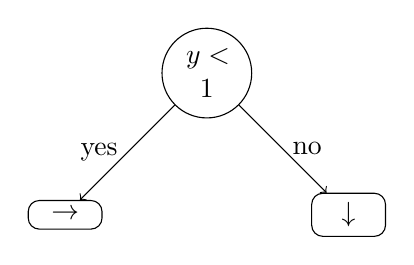
\begin{tikzpicture}[
    scale=1.2,
    decision/.style={circle, draw, text width=1.5em, text centered, minimum height=2.5em},
    action/.style={rectangle, draw, text width=2em, text centered, rounded corners}
]
    % Decision node
    \node[decision] (decide) at (0,0) {$y<1$};
    
    % Action nodes
    \node[action] (right) at (1.5,-1.5) {$\downarrow$};
    \node[action] (left) at (-1.5,-1.5) {$\rightarrow$};
    
    % Connections and labels
    \draw[->] (decide) -- node[right] {no} (right);
    \draw[->] (decide) -- node[left] {yes} (left);
\end{tikzpicture}
\caption{A simple decision tree policy based only on the $y$-coordinate. If $y < 1$, move right; otherwise, move down.}\label{fig:dt-simple}
\end{figure}

\begin{figure}[ht]
\centering
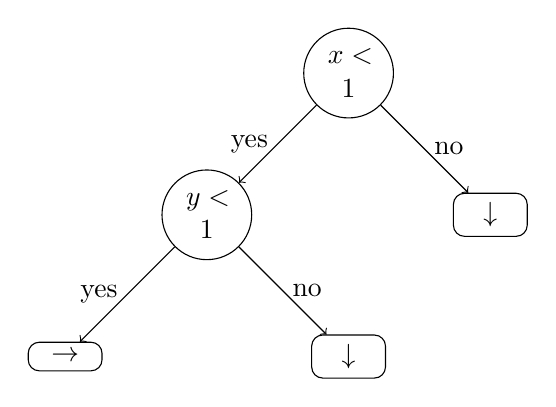
\begin{tikzpicture}[
    scale=1.2,
    decision/.style={circle, draw, text width=1.5em, text centered, minimum height=2.5em},
    action/.style={rectangle, draw, text width=2em, text centered, rounded corners}
]
    % Decision node
    \node[decision] (decide) at (0,0) {$x<1$};
    
    % Action nodes
    \node[action] (right) at (1.5,-1.5) {$\downarrow$};
    \node[decision] (decide2) at (-1.5,-1.5) {$y<1$};
    \node[action] (right2) at (0,-3) {$\downarrow$};
    \node[action] (left2) at (-3,-3) {$\rightarrow$};
    
    % Connections and labels
    \draw[->] (decide) -- node[right] {no} (right);
    \draw[->] (decide) -- node[left] {yes} (decide2);
    \draw[->] (decide2) -- node[left] {yes} (left2);
    \draw[->] (decide2) -- node[right] {no} (right2);
\end{tikzpicture}
\caption{A more complex decision tree policy with hierarchical decisions based on both $x$ and $y$ coordinates. This tree more closely approximates the optimal policy.}\label{fig:dt-complex}
\end{figure}

\begin{figure}[ht]
\centering
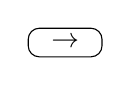
\begin{tikzpicture}[
    scale=1.2,
    decision/.style={circle, draw, text width=1.5em, text centered, minimum height=2.5em},
    action/.style={rectangle, draw, text width=2em, text centered, rounded corners}
]
    % Decision node
    \node[action] (decide) at (0,0) {$\rightarrow$};
\end{tikzpicture}
\caption{A trivial single-action policy that always selects the rightward action, regardless of the agent's position.}\label{fig:dt-trivial}
\end{figure}

\subsection{An objective function}

\subsection{Value of the optimal policy}

Let's compute the expected value of the optimal policy shown in Figure~\ref{fig:optimal-policy}, assuming a discount factor $\gamma \in (0,1)$. We'll first calculate the value function for each state under the optimal policy, then take the expectation over all possible starting states.

For the goal state $G$, where the agent always moves right and receives a reward of 1:
\begin{align}
V(G) &= 1 + \gamma V(G) \\
\Rightarrow V(G) &= \frac{1}{1-\gamma}
\end{align}

For state $S_2$, which transitions to $G$ with the down action:
\begin{align}
V(S_2) &= 0 + \gamma V(G) = \frac{\gamma}{1-\gamma}
\end{align}

For state $S_0$, which transitions to $G$ with the right action:
\begin{align}
V(S_0) &= 0 + \gamma V(G) = \frac{\gamma}{1-\gamma}
\end{align}

For state $S_1$, which transitions to $S_0$ with the down action:
\begin{align}
V(S_1) &= 0 + \gamma V(S_0) = \gamma \cdot \frac{\gamma}{1-\gamma} = \frac{\gamma^2}{1-\gamma}
\end{align}

Assuming a uniform distribution over starting states, the expected value is:
\begin{align}
\mathbb{E}[V] &= \frac{V(S_0) + V(S_1) + V(S_2) + V(G)}{4} \\
&= \frac{1}{4} \left( \frac{\gamma}{1-\gamma} + \frac{\gamma^2}{1-\gamma} + \frac{\gamma}{1-\gamma} + \frac{1}{1-\gamma} \right) \\
&= \frac{1}{4(1-\gamma)} \left( 1 + 2\gamma + \gamma^2 \right) \\
&= \frac{{(1 + \gamma)}^2}{4(1-\gamma)}
\end{align}

This expected value increases as $\gamma$ approaches 1, reflecting the growing importance of future rewards in the discounted cumulative reward objective.

\subsection{The decision tree policies values}
\begin{align}
J(T_0) &= \frac{1}{4}\sum_{i=0}^\infty \gamma^i + \frac{1}{4}\sum_{i=1}^\infty \gamma^i \\
&= \frac{1}{4} \cdot \frac{1}{1-\gamma} + \frac{1}{4} \cdot \frac{\gamma}{1-\gamma} \\
&= \frac{1 + \gamma}{4(1-\gamma)}
\end{align}

\begin{align}
J(T_1) &= \frac{1}{4} \left(\sum_{i=1}^\infty \gamma^{2i-1} + \sum_{i=0}^\infty\gamma^{2i}\zeta\right) + \frac{2}{4} \left(\sum_{i=2}^\infty \gamma^{2i-1} + \sum_{i=0}^\infty\gamma^{2i}\zeta\right) \\
&\quad + \frac{1}{4} \left(\sum_{i=3}^\infty \gamma^{2i-1} + \sum_{i=0}^\infty\gamma^{2i}\zeta\right) \\
&= \frac{1}{4} \left(\frac{\gamma}{1-\gamma^2} + \zeta\frac{1}{1-\gamma^2}\right) + \frac{2}{4} \left(\frac{\gamma^3}{1-\gamma^2} + \zeta\frac{1}{1-\gamma^2}\right) \\
&\quad + \frac{1}{4} \left(\frac{\gamma^5}{1-\gamma^2} + \zeta\frac{1}{1-\gamma^2}\right) \\
&= \frac{1}{4(1-\gamma^2)} \left[\gamma + \zeta + 2\gamma^3 + 2\zeta + \gamma^5 + \zeta\right] \\
&= \frac{1}{4(1-\gamma^2)} \left[\gamma + 2\gamma^3 + \gamma^5 + 4\zeta\right]
\end{align}

\begin{align}
J(T_2) &= \frac{1}{4} \left(\sum_{i=1}^\infty \gamma^{2i-1} + \sum_{i=0}^\infty\gamma^{2i}\zeta\right) + \frac{1}{4} \left(\sum_{i=2}^\infty \gamma^{2i-1} + \sum_{i=0}^\infty\gamma^{2i}\zeta\right) \\
&\quad + \frac{1}{4} \left(\sum_{i=2}^\infty\gamma^{3i-1} + \sum_{i=0}^\infty\gamma^{3i}\zeta + \sum_{i=1}^\infty\gamma^{3i-2}\zeta\right) \\
&\quad + \frac{1}{4} \left(\sum_{i=3}^\infty\gamma^{3i-1} + \sum_{i=0}^\infty\gamma^{3i}\zeta + \sum_{i=1}^\infty\gamma^{3i-2}\zeta\right) \\
&= \frac{1}{4} \left(\frac{\gamma}{1-\gamma^2} + \zeta\frac{1}{1-\gamma^2}\right) + \frac{1}{4} \left(\frac{\gamma^3}{1-\gamma^2} + \zeta\frac{1}{1-\gamma^2}\right) \\
&\quad + \frac{1}{4} \left(\frac{\gamma^5}{1-\gamma^3} + \frac{\zeta}{1-\gamma^3} + \frac{\zeta\gamma}{1-\gamma^3}\right) \\
&\quad + \frac{1}{4} \left(\frac{\gamma^8}{1-\gamma^3} + \frac{\zeta}{1-\gamma^3} + \frac{\zeta\gamma}{1-\gamma^3}\right) \\
&= \frac{1}{4} \left[\frac{\gamma + \gamma^3 + 2\zeta}{1-\gamma^2} + \frac{\gamma^5 + \gamma^8 + 2\zeta + 2\zeta\gamma}{1-\gamma^3}\right]
\end{align}
    
Let's determine the bounds on $\zeta$ such that $J(T_0) \leq J(T_1)$ and $J(T_2) \leq J(T_1)$.

\begin{align}
\text{For } J(T_0) \leq J(T_1): \\
\frac{1 + \gamma}{4(1-\gamma)} &\leq \frac{1}{4(1-\gamma^2)} \left[\gamma + 2\gamma^3 + \gamma^5 + 4\zeta\right] \\
\frac{(1 + \gamma)}{(1-\gamma)} &\leq \frac{\gamma + 2\gamma^3 + \gamma^5 + 4\zeta}{(1-\gamma^2)} \\
\frac{(1 + \gamma)}{(1-\gamma)} &\leq \frac{\gamma + 2\gamma^3 + \gamma^5 + 4\zeta}{(1-\gamma)(1+\gamma)} \\
(1 + \gamma)^2 &\leq \gamma + 2\gamma^3 + \gamma^5 + 4\zeta \\
1 + 2\gamma + \gamma^2 &\leq \gamma + 2\gamma^3 + \gamma^5 + 4\zeta \\
1 + \gamma + \gamma^2 - 2\gamma^3 - \gamma^5 &\leq 4\zeta \\
\zeta &\geq \frac{1 + \gamma + \gamma^2 - 2\gamma^3 - \gamma^5}{4}
\end{align}

\begin{align}
\text{For } J(T_2) \leq J(T_1): \\
\end{align}

For $J(T_2) \leq J(T_1)$, we need to compare:
\begin{align}
\frac{1}{4} &\left[\frac{\gamma + \gamma^3 + 2\zeta}{1-\gamma^2} + \frac{\gamma^5 + \gamma^8 + 2\zeta + 2\zeta\gamma}{1-\gamma^3}\right] \\
&\leq \frac{1}{4(1-\gamma^2)} \left[\gamma + 2\gamma^3 + \gamma^5 + 4\zeta\right]
\end{align}

For $J(T_2) \leq J(T_1)$, I'll proceed with a more detailed derivation:

\begin{align}
\frac{1}{4} &\left[\frac{\gamma + \gamma^3 + 2\zeta}{1-\gamma^2} + \frac{\gamma^5 + \gamma^8 + 2\zeta + 2\zeta\gamma}{1-\gamma^3}\right] \leq \frac{1}{4(1-\gamma^2)} \left[\gamma + 2\gamma^3 + \gamma^5 + 4\zeta\right]
\end{align}

Let's first work on the left side to find a common denominator $(1-\gamma^2)(1-\gamma^3)$:

\begin{align}
\frac{1}{4} &\left[\frac{(\gamma + \gamma^3 + 2\zeta)(1-\gamma^3)}{(1-\gamma^2)(1-\gamma^3)} + \frac{(\gamma^5 + \gamma^8 + 2\zeta + 2\zeta\gamma)(1-\gamma^2)}{(1-\gamma^2)(1-\gamma^3)}\right] \\
&= \frac{1}{4(1-\gamma^2)(1-\gamma^3)}\left[(\gamma + \gamma^3 + 2\zeta)(1-\gamma^3) + (\gamma^5 + \gamma^8 + 2\zeta + 2\zeta\gamma)(1-\gamma^2)\right]
\end{align}

Let's expand these terms:
\begin{align}
(\gamma + \gamma^3 + 2\zeta)(1-\gamma^3) &= \gamma - \gamma^4 + \gamma^3 - \gamma^6 + 2\zeta - 2\zeta\gamma^3 \\
(\gamma^5 + \gamma^8 + 2\zeta + 2\zeta\gamma)(1-\gamma^2) &= \gamma^5 - \gamma^7 + \gamma^8 - \gamma^{10} + 2\zeta - 2\zeta\gamma^2 + 2\zeta\gamma - 2\zeta\gamma^3
\end{align}

Now the right side:
\begin{align}
\frac{1}{4(1-\gamma^2)} \left[\gamma + 2\gamma^3 + \gamma^5 + 4\zeta\right] &= \frac{(1-\gamma^3)(\gamma + 2\gamma^3 + \gamma^5 + 4\zeta)}{4(1-\gamma^2)(1-\gamma^3)}
\end{align}

Expanding:
\begin{align}
(1-\gamma^3)(\gamma + 2\gamma^3 + \gamma^5 + 4\zeta) &= \gamma - \gamma^4 + 2\gamma^3 - 2\gamma^6 + \gamma^5 - \gamma^8 + 4\zeta - 4\zeta\gamma^3
\end{align}

Our inequality now becomes:
\begin{align}
&\frac{1}{4(1-\gamma^2)(1-\gamma^3)}\left[(\gamma - \gamma^4 + \gamma^3 - \gamma^6 + 2\zeta - 2\zeta\gamma^3) + (\gamma^5 - \gamma^7 + \gamma^8 - \gamma^{10} + 2\zeta - 2\zeta\gamma^2 + 2\zeta\gamma - 2\zeta\gamma^3)\right] \\
&\leq \frac{1}{4(1-\gamma^2)(1-\gamma^3)}\left[\gamma - \gamma^4 + 2\gamma^3 - 2\gamma^6 + \gamma^5 - \gamma^8 + 4\zeta - 4\zeta\gamma^3\right]
\end{align}

Multiplying both sides by $4(1-\gamma^2)(1-\gamma^3)$ and grouping terms:
\begin{align}
&\gamma - \gamma^4 + \gamma^3 - \gamma^6 + 2\zeta - 2\zeta\gamma^3 + \gamma^5 - \gamma^7 + \gamma^8 - \gamma^{10} + 2\zeta - 2\zeta\gamma^2 + 2\zeta\gamma - 2\zeta\gamma^3 \\
&\leq \gamma - \gamma^4 + 2\gamma^3 - 2\gamma^6 + \gamma^5 - \gamma^8 + 4\zeta - 4\zeta\gamma^3
\end{align}

Canceling like terms and rearranging:
\begin{align}
&\gamma^3 - \gamma^7 + \gamma^8 - \gamma^{10} + 4\zeta - 2\zeta\gamma^2 + 2\zeta\gamma \\
&\leq 2\gamma^3 - 2\gamma^6 - \gamma^8
\end{align}

Further simplifying:
\begin{align}
&\gamma^3 - \gamma^7 + \gamma^8 - \gamma^{10} - 2\zeta\gamma^2 + 2\zeta\gamma \\
&\leq 2\gamma^3 - 2\gamma^6 - \gamma^8
\end{align}

Rearranging to isolate $\zeta$:
\begin{align}
2\zeta\gamma^2 - 2\zeta\gamma &\leq 2\gamma^3 - \gamma^3 + \gamma^7 - \gamma^8 - 2\gamma^6 + \gamma^8 + \gamma^{10} \\
2\zeta\gamma(\gamma - 1) &\leq \gamma^3 - 2\gamma^6 + \gamma^7 + \gamma^{10} \\
\end{align}

Since $\gamma - 1 < 0$ (as $0 < \gamma < 1$), we flip the inequality when dividing:
\begin{align}
2\zeta\gamma &\geq \frac{\gamma^3 - 2\gamma^6 + \gamma^7 + \gamma^{10}}{1 - \gamma} \\
\zeta &\geq \frac{\gamma^3 - 2\gamma^6 + \gamma^7 + \gamma^{10}}{2\gamma(1 - \gamma)} \\
\zeta &\geq \frac{\gamma^2(1 - 2\gamma^3 + \gamma^4 + \gamma^7)}{2(1 - \gamma)}
\end{align}

This can be rewritten in a cleaner form as:
\begin{align}
\zeta &\geq \frac{\gamma^2(1 - 2\gamma^3 + \gamma^4 + \gamma^7)}{2(1 - \gamma)}
\end{align}

This gives us our bound for $\zeta$ to ensure $J(T_2) \leq J(T_1)$.

Combining both conditions, $\zeta$ must satisfy:
\begin{align}
\zeta \geq \max\left\{\frac{1 + \gamma + \gamma^2 - 2\gamma^3 - \gamma^5}{4}, \frac{\gamma^2(1 - 2\gamma^3 + \gamma^4 + \gamma^7)}{2(1 - \gamma)}\right\}
\end{align}

\begin{figure}[ht]
\centering
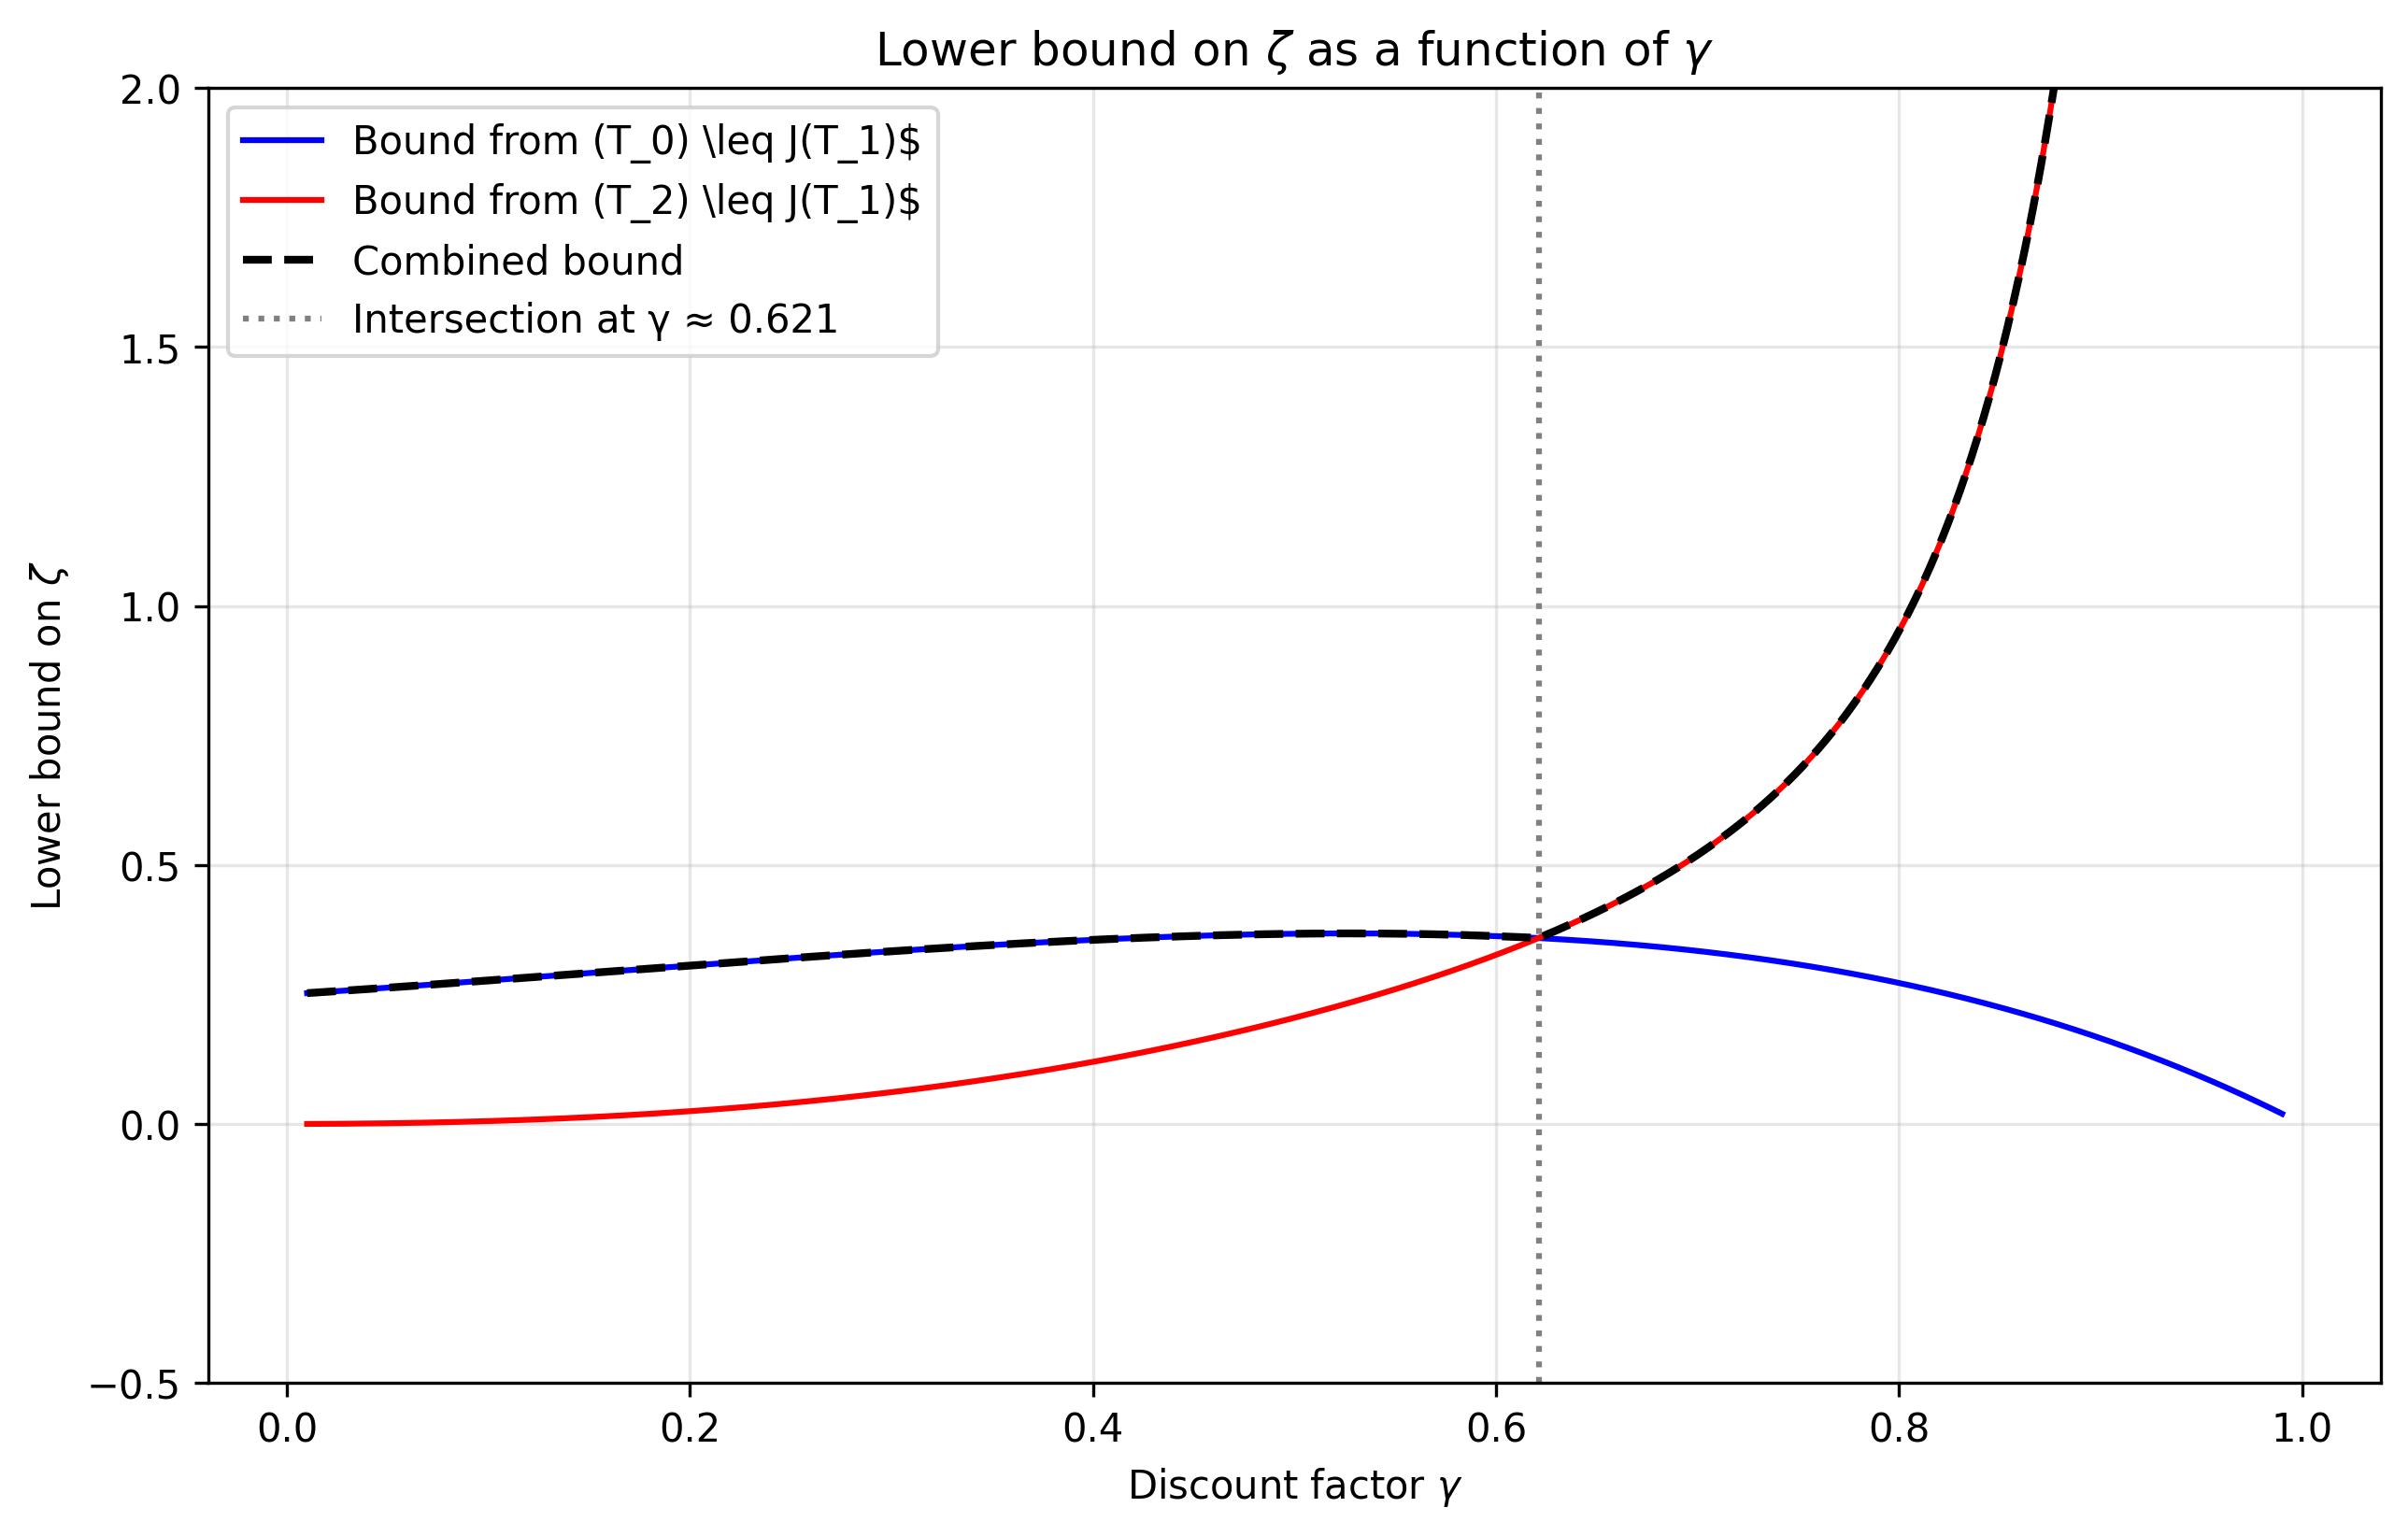
\includegraphics[width=0.8\textwidth]{zeta_bound_plot.png}
\caption{Plot of the lower bound on $\zeta$ as a function of the discount factor $\gamma$. The blue line represents the bound from $J(T_0) \leq J(T_1)$, the red line represents the bound from $J(T_2) \leq J(T_1)$, and the black dashed line shows the combined bound (maximum of the two).}
\label{fig:zeta-bound}
\end{figure}

Figure~\ref{fig:zeta-bound} illustrates how these bounds vary with the discount factor $\gamma$. For smaller values of $\gamma$, the bound from $J(T_0) \leq J(T_1)$ dominates, while for larger values of $\gamma$, the bound from $J(T_2) \leq J(T_1)$ becomes more restrictive.

\subsection{The interpretability-performance trade-off}

\section{A Reinforcement Learning experiment}

